\chapter{Instalacija dSPACE programa}\label{dSpace}

\qquad Za razvoj upravljačkog algoritma korištenjem \textit{MicroLabBox} razvojnog sistema je potrebno instalirati \textit{dSPACE} softver koji će se integrirati sa \textit{Matlab/Simulink} okruženjem. U nastavku će biti dat proces instalacije \textit{dSPACE} programskog paketa, verzije \textbf{2018-A}.

\section{Tekstualni i video vodič za instalaciju}

\qquad Na zvaničnoj stranici proizvođača je moguće pronaći tekstualne (\textit{.pdf}) \cite{dSPACEinstall} i video \cite{dSPACEvideo} instrukcije za instalaciju \textit{dSPACE} softvera.

\section{Datoteke za instalaciju softvera}\label{folder}

\qquad Uz \textit{MicroLabBox} razvojni sistem dolaze dva DVD-a, na kojima se nalaze datoteke potrebne za instalaciju softvera. Detaljna uputstva za instalaciju se nalaze u datoteci \textbf{InstallingdSPACESoftware.pdf}. 

Vlasnici dSPACE licence i registrirani korisnici softver mogu preuzeti preko \href{https://www.dspace.com/en/pub/home/support/patches/rlsdl.cfm}{linka} koji vodi do zvanične internet stranice proizvođača. Pogodan način za instalaciju podrazumijeva kopiranje sadržaja sa oba DVD-a u isti folder na računaru, pri čemu je potrebno izvršiti prepisivanje (\textit{engl. overwrite}) odgovarajućih datoteka.

\section{Kompatibilne Matlab/Simulink distribucije}

\qquad dSPACE verzije 2018-A sadrži sljedeće programske komponente sa pripadajućim verzijama:

\begin{enumerate}
	\item RCP and HIL Software,
	\item AutomationDesk 5.6,
	\item TargetLink 4.3,
	\item Model Compare 2.8,
	\item dSPACE Python Extensions 2.5 i
	\item XIL API .NET MAPort 2018-A.
\end{enumerate}

Sve navedene komponente su kompatibilne sa \textit{Matlab} distribucijama \textbf{R2016b}, \textbf{R2017a} i \textbf{R2017b}. Djelimična kompatibilnost sa gorenavedenim programima se ostvaruje kroz distribucije R2016a (podržane stavke 3 i 4) i R2018a (podržane stavke: 1, 2, 5 i 6).

\section{Dodatne postavke}

\qquad Prije pokretanja instalacije \textit{dSPACE} softvera, potrebno je isključiti antivirusnu zaštitu i vatrozid (\textit{engl. firewall}) na računaru, kao i obezbjediti putem opcija za štednju energije (\textit{engl. power saving options}) da se računar neće isključiti ili preći u režim mirovanja (\textit{engl. sleep mode}) tokom procesa instalacije.

Također, potrebno je instalirati \textbf{MATLAB Support for MinGW-w64 C/C++ Compiler}, koji je moguće pronaći u \textit{Get Add-Ons} sekciji \textit{Matlabovog} korisničkog sučelja i \textbf{.NET Framework 3.5}.

\section{Proces instalacije dSPACE softvera}

\qquad Prije same instalacije je potrebno zatvoriti sve pokrenute programe. Kao što je navedeno u sekciji \ref{folder}, sadržaj sa oba DVD-a je pogodno kopirati u isti folder na računaru na koji se planira instalirati dSPACE i sa te lokacije \textbf{pokrenuti} instalaciju.

\subsection{Pokretanje instalacije}\label{pokretanje.instalacije}

\qquad Proces instalacije se započinje pokretanjem \textbf{Install\_Release.exe} datoteke. Pojavljuje se dijaloški okvir, prikazan na slici (\ref{fig:welcome}).

\begin{figure}[h]
\begin{center}
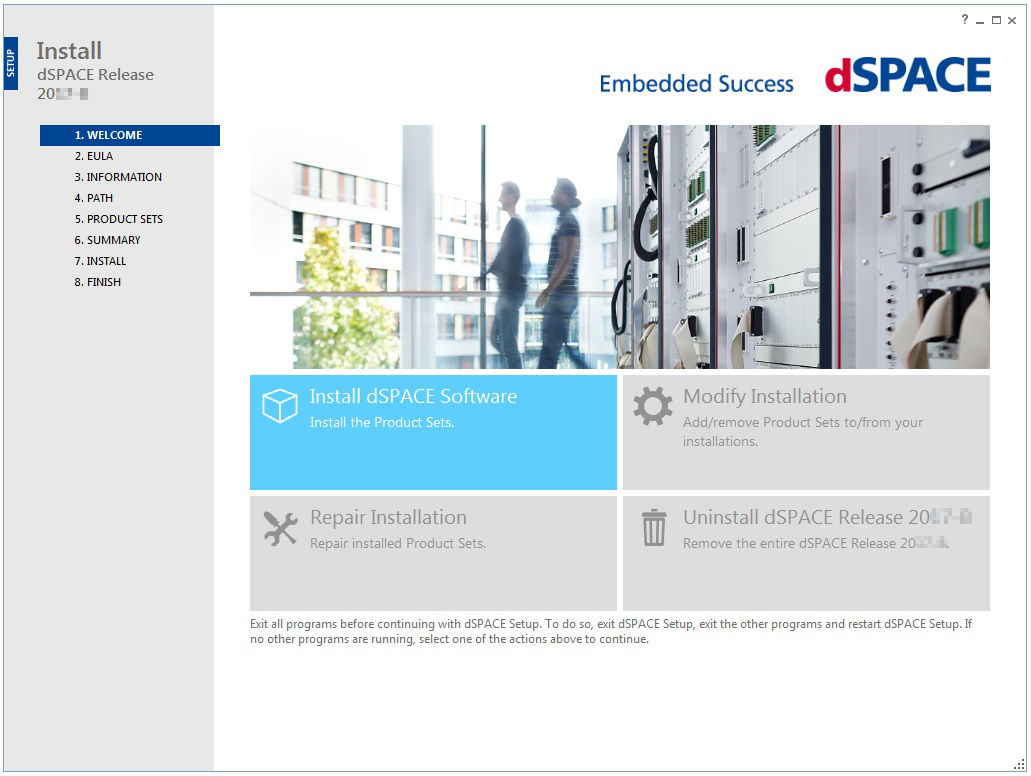
\includegraphics[width=\textwidth]{slike/dSpace/welcome.png}
\end{center}
\caption{Dijaloški okvir koji se pojavljuje nakon pokretanja instalacije \cite{dSPACEinstall}}
\label{fig:welcome}
\end{figure}

\textit{Napomena: \textit{dSPACE} od korisnika može tražiti ponovno pokretanje računara prije početka instalacije. Tada je potrebno \textit{restartovati} računar i vratiti se na korak \ref{pokretanje.instalacije}.}

\subsection{Instalacija, modifikacija, brisanje i popravljanje dSPACE softvera}

\qquad Dostupne opcije u dijaloškom okviru, koji je prikazan na slici \ref{fig:welcome}, mogu biti različite u zavisnosti od toga da li je na računaru već instaliran \textit{dSPACE} softver. Moguće opcije su:

\begin{itemize}
	\item Install \textit{dSPACE} Software - instalacija programa
	\item Modify Installation - dodavanje/brisanje dijelova programa iz već postojeće instalacije
	\item Repair Installation - popravljanje dijelova programa
	\item Uninstall \textit{dSPACE} Release 20$xx-x$ - brisanje svih instaliranih dijelova programa
\end{itemize}

Ukoliko na računaru nije već instaliran \textit{dSPACE}, jedina opcija koju je potrebno i moguće odabrati je \textbf{Install dSPACE Software}.

Nakon toga je potrebno \textbf{specificirati lokaciju} na kojoj će se instalirati \textit{dSPACE}. Pojavljuje se prozor prikazan na slici (\ref{fig:product.sets}).

\begin{figure}[h]
\begin{center}
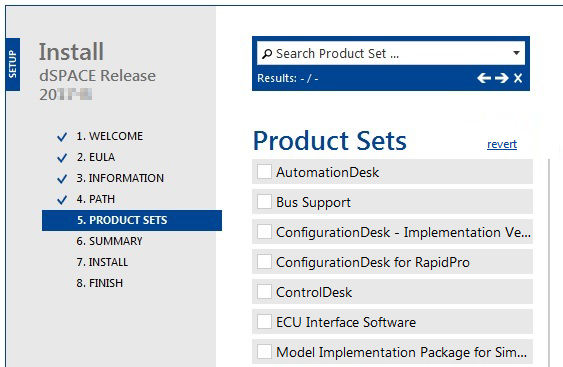
\includegraphics[width=\textwidth]{slike/dSpace/product sets.png}
\end{center}
\caption{Izbor dijelova programa za instalaciju \citep{dSPACEinstall}}
\label{fig:product.sets}
\end{figure}

\subsection{Instalacija dijelova programa}

\qquad U dijaloškom okviru, prikazanom na slici (\ref{fig:product.sets}), moguće je odabrati koji će se \textit{dSPACE} programski paketi instalirati na računar. Nakon što korisnik odabere željene pakete, potrebno je kliknuti na dugme \textbf{Next} u istom prozoru.

\subsection{Summary page}

\qquad Otvara se \textit{Summary page}, gdje je moguće odabrati sljedeće opcije:

\begin{itemize}
	\item Shut down after installation - Isključivanje računara nakon instalacije
	\item Start Installation Manager after installation - Pokretanje \textit{Installation Manager} programa nakon instalacije
\end{itemize}

Odabrati željene opcije i kliknuti na dugme \textbf{Start}.

\subsection{Završetak instalacije}

\qquad Potrebno je da korisnik izvrši ponovno pokretanje računara, kada to od njega instalacioni program bude tražio.

\subsection{Preuzimanje i instaliranje zakrpa}

\qquad Eventualne greške u instaliranom softveru se ispravljaju odgovarajućim zakrpama (\textit{engl. patches}) i ažuriranjima (\textit{engl. updates}). Na zvaničnoj stranici proizvođača \citep{dSPACEpatch} je moguće pronaći listu svih zakrpi i ažuriranja za odgovarajuću verziju \textit{dSPACE} softvera. Potrebno je \textbf{preuzeti} i \textbf{instalirati} date zakrpe.

\textit{Napomena: Pojedina ažuriranja i zakrpe zahtijevaju validni \textit{Software Maintenance Service} za preuzimanje i instalaciju.}

\section{Integracija dSPACE softvera sa Matlab/Simulink razvojnim okruženjem}

\qquad Instalirani \textit{dSPACE} softver je potrebno integrirati i povezati sa \textit{Matlab/Simulink} programskim paketom. To je moguće učiniti pomoću programa \textbf{dSPACE Installation Manager}.

Pokretanjem istog i navigacijom do \textbf{MATLAB} kartice (\textit{engl. tab}), dolazi se do prozora na kojem su prikazane sve \textit{Matlab} distribucije instalirane na računaru. \textit{dSPACE} je integriran sa odgovarajućom \textit{Matlab} distribucijom ukoliko se pored oznake \textbf{dSPACE Software Integration} nalazi \textit{integrated}, kao na slici (\ref{fig:matlab-integrate}).

\begin{figure}[h]
\begin{center}
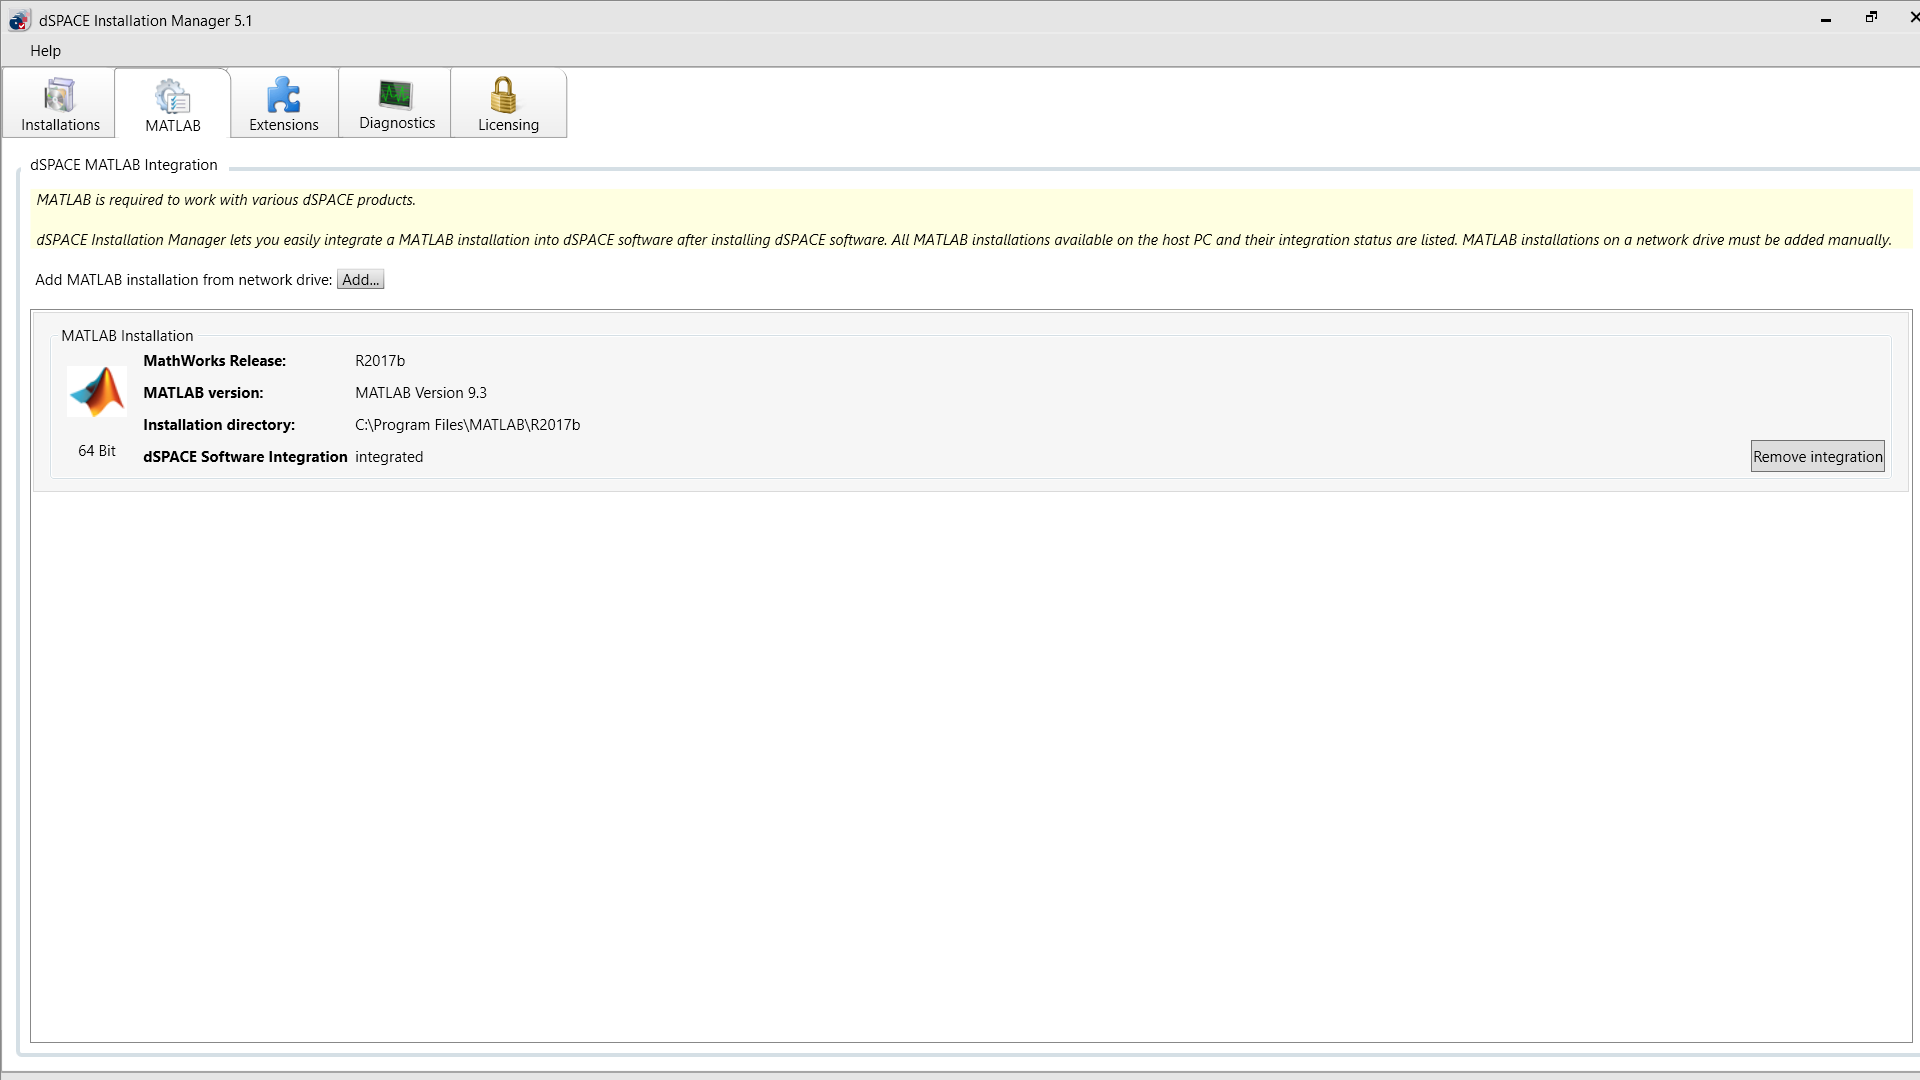
\includegraphics[width=\textwidth]{slike/dSpace/matlab-integrate.png}
\end{center}
\caption{Integracija \textit{dSPACE} instalacije sa odgovarajućom \textit{Matlab} distribucijom}
\label{fig:matlab-integrate}
\end{figure}

Pored integracije, potrebno je povezati (\textit{engl. connect}) dSPACE instalaciju sa odgovarajućom \textit{Matlab} distribucijom. U \textbf{dSPACE Installation Manager} programu je potrebno kroz \textit{Installations} i \textit{Installation Overview} kartice za svaku programsku komponentu, kod koje je dostupna ta opcija, u kartici \textit{Connect to MATLAB Release} - označiti (\textit{engl. check}) \textit{Connected} za odgovarajuću Matlab distribuciju, kao na slici (\ref{fig:matlab-connect}).

\begin{figure}[h]
\begin{center}
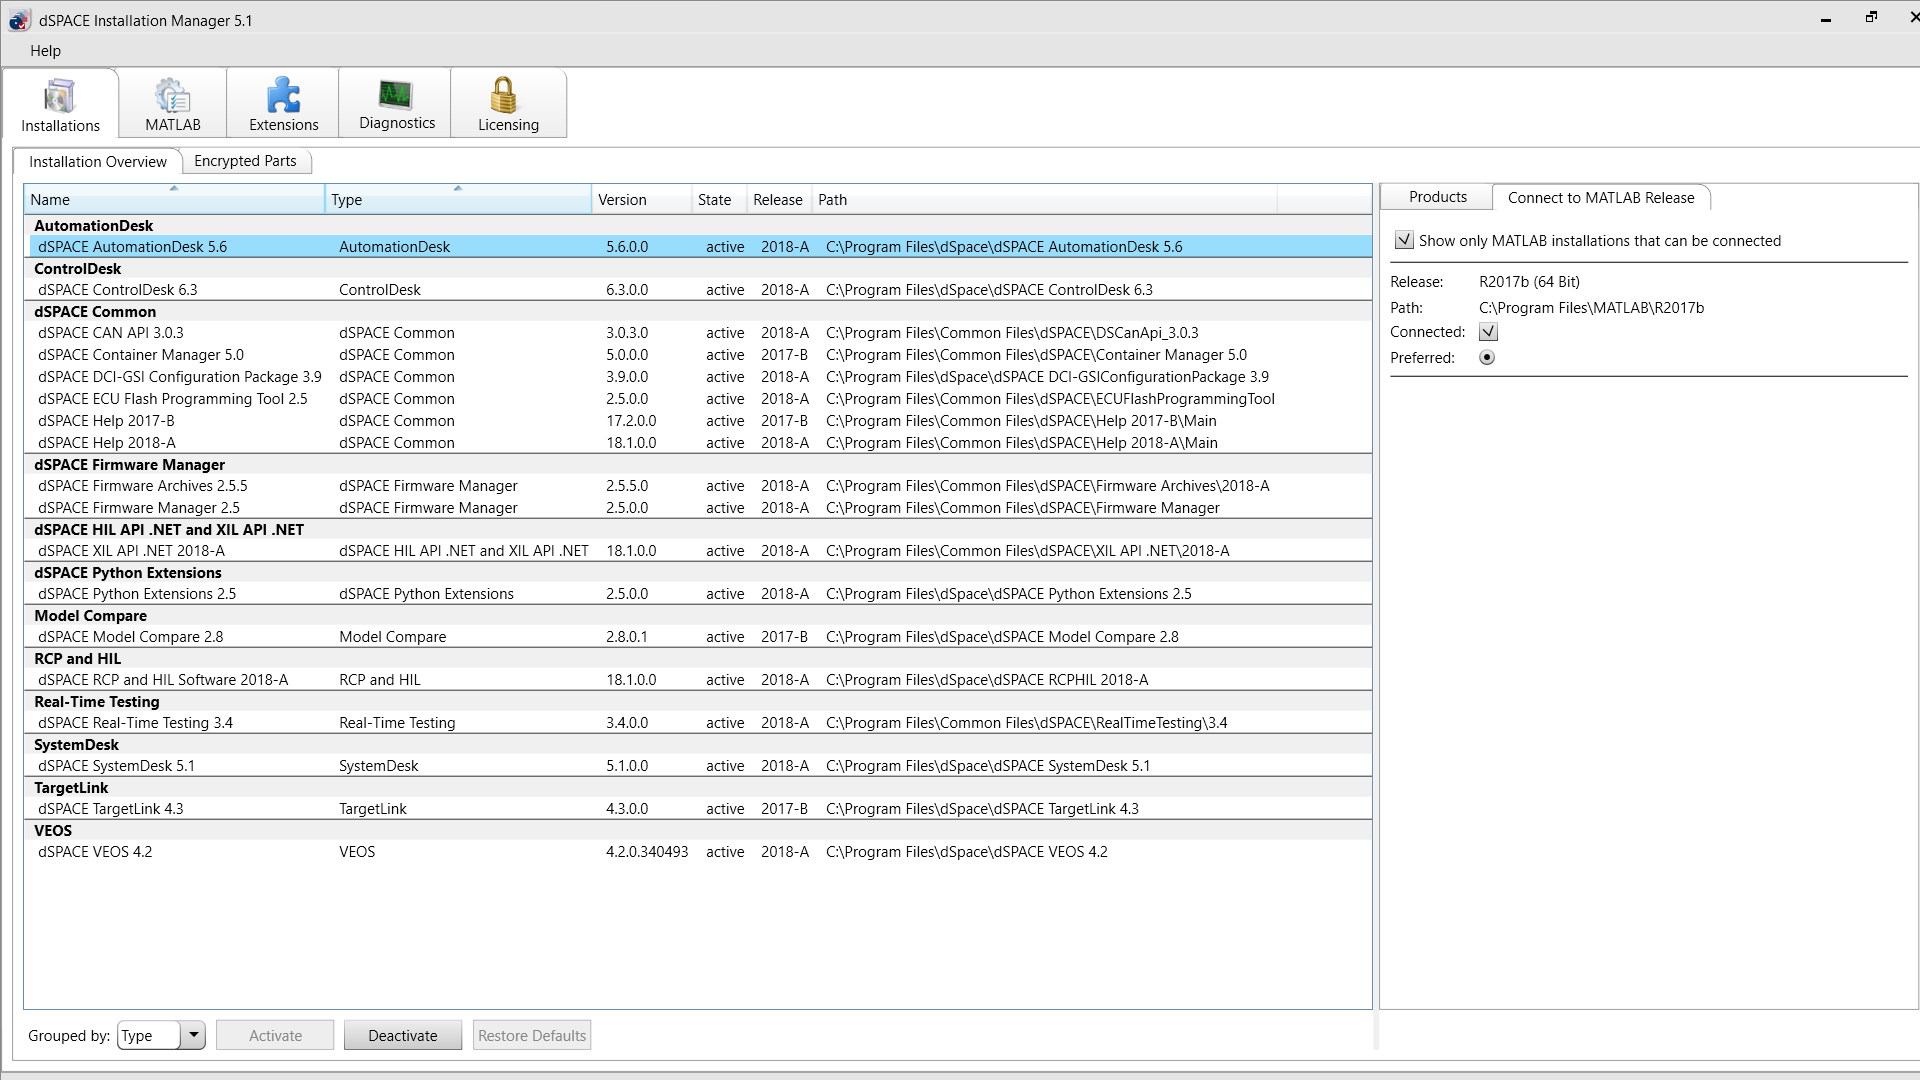
\includegraphics[width=\textwidth]{slike/dSpace/matlab-connect.png}
\end{center}
\caption{Povezivanje \textit{dSPACE} instalacije sa odgovarajućom \textit{Matlab} distribucijom}
\label{fig:matlab-connect}
\end{figure}

Prije pokretanja \textit{Matlab} distribucije, potrebno je zatvoriti dSPACE Installation Manager program sa ranije navedenom konfiguracijom. Programski paket \textit{Matlab} će pri pokretanju izvršiti \textit{konfiguraciju} dSPACE softvera, kao što je prikazano na slici (\ref{fig:matlab-configure}).

\begin{figure}[h]
\begin{center}
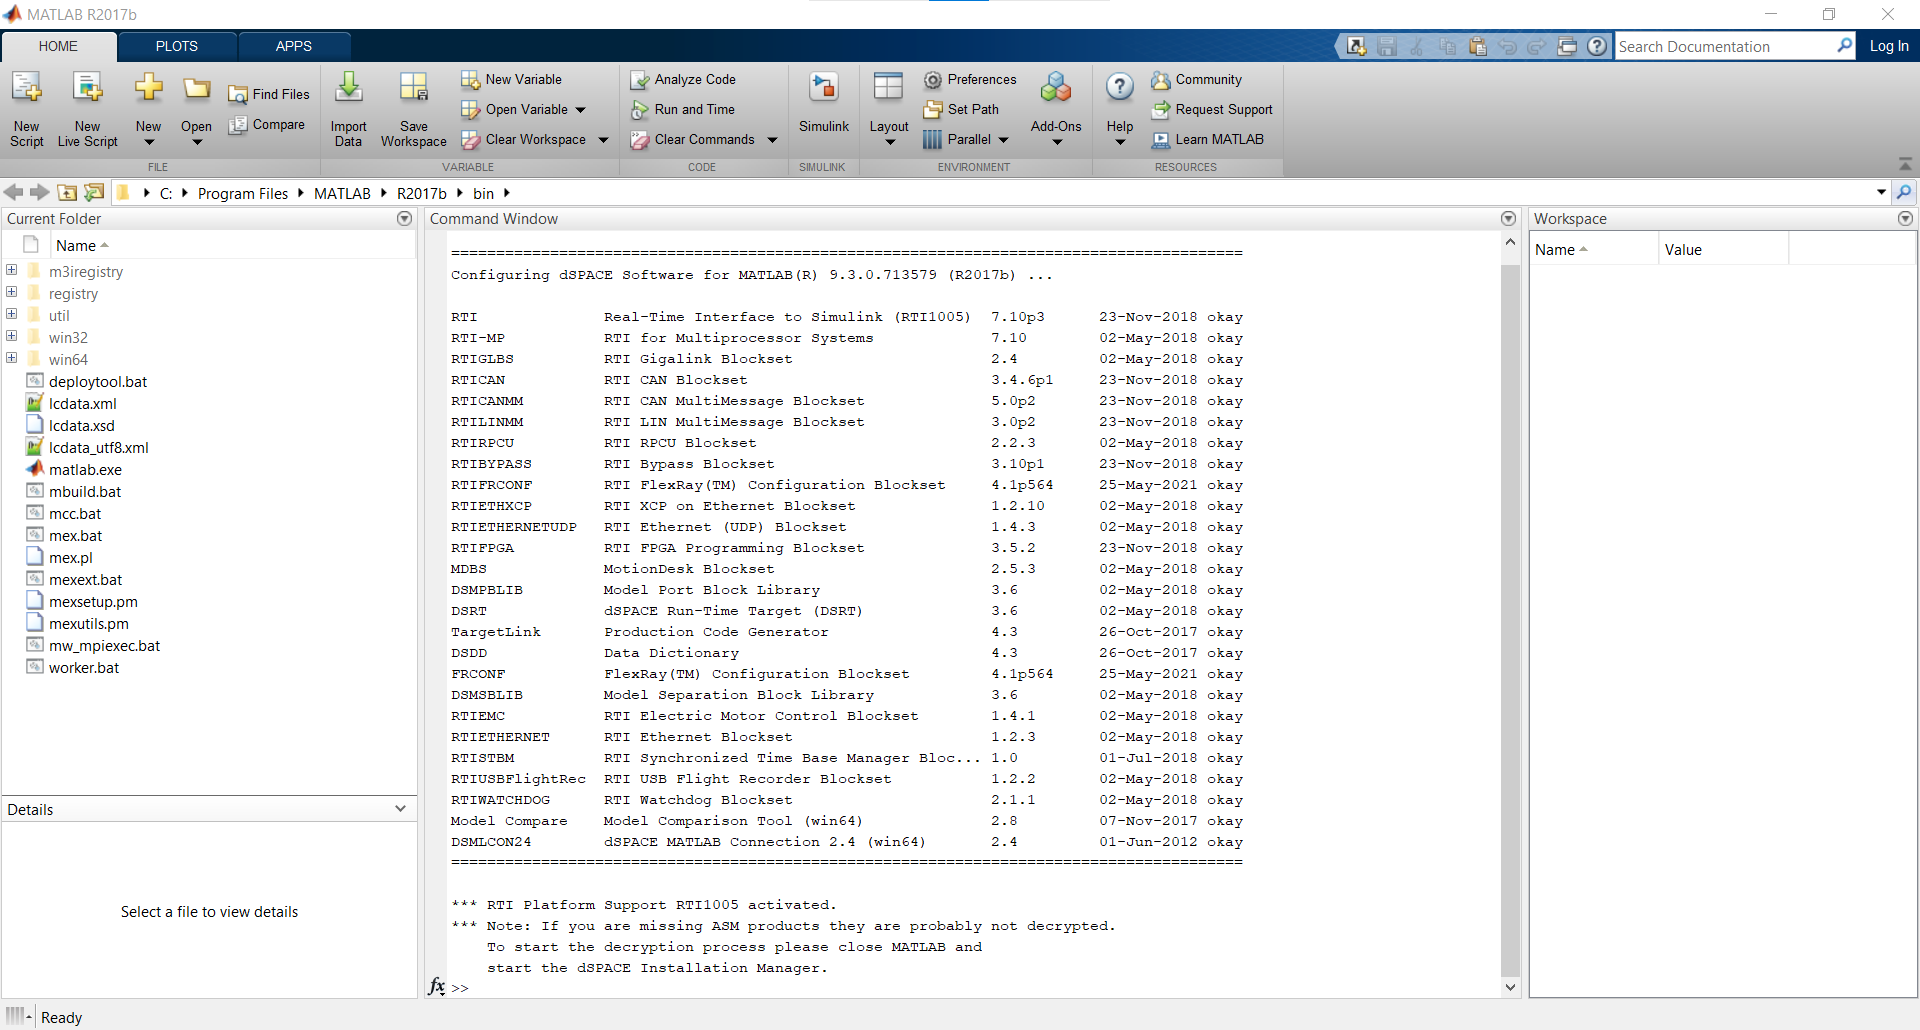
\includegraphics[width=\textwidth]{slike/dSpace/matlab-configure.png}
\end{center}
\caption{Konfiguracija \textit{dSPACE} softvera prilikom pokretanja Matlab distribucije}
\label{fig:matlab-configure}
\end{figure}

\section{Licenciranje i dekripcija dSPACE softvera}